\documentclass[10pt,twocolumn]{article}

\usepackage[margin=1in]{geometry}
\usepackage{amsmath,amssymb}
\usepackage{graphicx}
\usepackage{booktabs}
\usepackage{colortbl}
\usepackage{hyperref}
\usepackage{xcolor}
\usepackage[protrusion=true,expansion=false]{microtype}
\usepackage{listings}
\usepackage{caption}
\usepackage{subcaption}
\usepackage{abstract}
\usepackage{titlesec}
\usepackage{parskip}
\usepackage{fancyhdr}
\usepackage{natbib}
\usepackage[section]{placeins}  % FloatBarrier at every \section

\definecolor{codegray}{rgb}{0.95,0.95,0.95}
\definecolor{codeblue}{rgb}{0.1,0.2,0.6}

\lstset{
  backgroundcolor=\color{codegray},
  basicstyle=\ttfamily\small,
  keywordstyle=\color{codeblue}\bfseries,
  language=Python,
  frame=single,
  framerule=0pt,
  breaklines=true,
  captionpos=b,
}

\hypersetup{
  colorlinks=true,
  linkcolor=codeblue,
  citecolor=codeblue,
  urlcolor=codeblue,
}

\pagestyle{fancy}
\fancyhf{}
\rhead{\small Adaptive Precision Attention}
\lhead{\small Chaithu Talasila}
\cfoot{\thepage}

\title{\textbf{Adaptive Precision Attention:\\
Evolutionary Discovery to Hardware-Verified Ratio Gates}}

\author{
  Chaithu Talasila\\
  \texttt{https://github.com/LonghornSilicon/attention-compute-unit}
}

\date{}

\begin{document}

\maketitle
\thispagestyle{fancy}

%------------------------------------------------------------------
\begin{abstract}
We present an evolutionary approach to discovering per-block precision
allocation policies for mixed-precision attention, then trace a complete
path from policy discovery to hardware-verified implementation.
Using OpenEvolve, an LLM-guided evolutionary search framework, we evolve a
precision policy over 14 per-block statistics and 6 precision levels.
The search converges on a two-threshold policy using softmax entropy and
outlier presence. We then show that entropy---which requires 32{,}000
transcendental operations per tile---is replaceable by a pre-softmax
ratio signal ($\max|S|/\mathrm{mean}|S|$) with 100\% decision agreement
and zero dangerous misses at threshold 10. The hardware implementation
requires no division: $\max \times N > 10 \times \mathrm{sum}$, a left
shift, two shifts-and-add for multiply-by-10, and one comparator.

Validated on real Qwen2/Qwen2.5 language models at 512-token sequences,
91--97\% of attention tiles are INT8-safe across model sizes from 0.5B
to 3B parameters (24--36 layers). INT8 safety \emph{improves} with scale:
the 1.5B model reaches 97.1\% INT8-safe tiles. Fixed-point simulation
confirms 100\% decision agreement at every tested bit width (4, 6, 8,
10, 12, 16 bits), with a 16-bit sum accumulator and 20-bit comparator
sufficient. The precision controller occupies a handful of logic gates
and 64 bytes of per-layer threshold registers---directly implementable
as an ASIC attention accelerator.
\end{abstract}

%------------------------------------------------------------------
\section{Introduction}

The attention mechanism is the computational core of transformer-based
language models, and its efficient implementation has been a sustained
focus of systems research. FlashAttention \citep{dao2022flashattention}
and its successors \citep{dao2023flashattention2,shah2024flashattention3}
achieve near-peak hardware utilization through tiled, fused computation
that avoids materializing the full $N \times N$ attention matrix.
FlashAttention-3 introduces FP8 quantization on Hopper GPUs, achieving
up to 1.2 PFLOPs/s, but treats precision as a global choice: all blocks
are computed at the same numerical format.

In practice, different blocks of the attention matrix have different
precision requirements. Blocks where the softmax distribution is peaked
and input values contain statistical outliers are sensitive to
quantization error. Blocks where attention is uniformly distributed are
robust to aggressive compression. This motivates \emph{adaptive precision
attention}, where each block is quantized to the minimum precision that
preserves output quality.

The challenge is determining which blocks need protection. We pose
precision allocation as a program synthesis problem and solve it with
evolutionary search over per-block statistics. We then carry the
discovered policy all the way to fixed-point hardware simulation,
validating that the signal survives real LLM activations and integer
arithmetic.

\paragraph{Contributions.}
\begin{itemize}
  \item An evolutionary framework for precision policy discovery over 14
  per-block statistics and 6 precision levels, converging on two
  comparisons and one AND gate.
  \item Proof that softmax entropy (32K transcendental ops/tile) is
  replaceable by a pre-softmax ratio signal using only a max tree, an
  adder tree, and one comparator---with 100\% agreement and zero
  dangerous misses.
  \item Real LLM validation on Qwen2-0.5B, Qwen2-1.5B, Qwen2.5-3B, and Phi-2 (2.7B):
  91--97\% of tiles are INT8-safe; INT8 coverage \emph{improves} with
  model scale.
  \item Fixed-point simulation confirming 100\% agreement at 4-bit score
  representation; hardware register budget of 16-bit sum + 20-bit
  comparator.
  \item A working Triton kernel prototype (12/12 correctness tests
  passing) and KV-cache module with uniform $2\times$ compression.
\end{itemize}

%------------------------------------------------------------------
\section{Related Work}

\paragraph{Efficient attention.}
FlashAttention \citep{dao2022flashattention} introduced tiled, IO-aware
attention computation. FlashAttention-2 \citep{dao2023flashattention2}
improved parallelism. FlashAttention-3 \citep{shah2024flashattention3}
targets Hopper GPUs with warp specialization and uniform FP8 block
quantization. All three treat precision as a global setting.

\paragraph{Adaptive quantization.}
\citet{boroujeni2026adaptive} propose per-token KV-cache quantization
with four precision levels selected by entropy and attention variance,
achieving 17.75\% latency reduction. SmoothQuant
\citep{xiao2023smoothquant} redistributes quantization difficulty between
activations and weights. GPTQ \citep{frantar2023gptq} uses second-order
information for weight quantization. Our work focuses on attention
computation precision using evolutionary search, targeting ASIC
implementation.

\paragraph{Program synthesis.}
OpenEvolve \citep{openevolve2025} extends FunSearch
\citep{romera2024funsearch} with multi-objective optimization and
island-based population management. We use it as the search engine with
Claude Sonnet as the LLM backbone.

%------------------------------------------------------------------
\section{Method}

\subsection{Problem Formulation}

We define a precision policy as a function mapping per-block statistics
to a precision level:
\begin{align*}
\text{policy}: \mathcal{S} \rightarrow \{&\texttt{fp16},\;\texttt{fp8\_e4m3},\;\texttt{fp8\_e5m2},\\
                                         &\texttt{int8},\;\texttt{fp4},\;\texttt{int4}\}
\end{align*}

For each query block $\mathbf{Q}_i$ and key-value block
$(\mathbf{K}_j, \mathbf{V}_j)$, we compute block statistics, query the
policy, and apply a quantize-dequantize roundtrip before accumulation
(always in FP32).

\subsection{Block Statistics}

For each block pair $(i,j)$ we extract 14 statistics: L2 norms of
$\mathbf{Q}$, $\mathbf{K}$, $\mathbf{V}$ blocks; statistics of
pre-softmax scores $\mathbf{S} = \mathbf{Q}\mathbf{K}^\top/\sqrt{d}$;
the Shannon entropy of the row-wise softmax; causal distance; block
indices; and an outlier flag:
\[
\texttt{has\_outlier} = \max|\mathbf{S}| > \mu_{|\mathbf{S}|} + 10\,\sigma_{|\mathbf{S}|}
\]

Block size is 128 tokens, matching FlashAttention-3's tile size.

\subsection{Evolutionary Search}

We use OpenEvolve \citep{openevolve2025} with 50 candidates across 3
islands, 80 iterations of diff-based mutation, Claude Sonnet (80\%) and
Haiku (20\%) as LLM backbone, and a fitness function weighting 50\%
accuracy ($1/(1 + \text{RMSE} \cdot 10)$ vs FP64) + 30\% compression +
20\% reliability.

\subsection{Evaluation Workloads}

We evaluate on 12 workloads spanning $N \in \{512, 2048, 4096, 8192\}$,
$d \in \{64, 128\}$, with and without causal masking, and with 0.1\% of
elements scaled by $100\times$ to simulate LLM activation outliers.

%------------------------------------------------------------------
\section{Results}

\subsection{Converged Policy}

After 80 iterations (combined score 0.745, target $>$0.65), the search
converged on:

\begin{lstlisting}[caption={Evolved precision policy (2 of 14 features used).}]
def precision_policy(block_stats):
    has_outlier = block_stats.get('has_outlier', False)
    entropy = block_stats.get('entropy', 4.3)
    if has_outlier and entropy < 2.0:
        return "fp16"
    return "int8"
\end{lstlisting}

All intermediate formats (FP8, FP4, INT4) were eliminated by the search.

\subsection{Accuracy vs.\ Baselines}

Table~\ref{tab:avg_results} summarises aggregate metrics.
Table~\ref{tab:results} gives per-workload detail.
Figure~\ref{fig:accuracy} shows the log-scale RMSE comparison.
On outlier workloads, uniform INT8 fails catastrophically (RMSE $>$ 1.0),
while the evolved policy matches FP16 exactly.

\begin{table}[tbp]
\centering
\caption{Average metrics across all 12 workloads.}
\label{tab:avg_results}
\small
\begin{tabular}{lrrc}
\toprule
Strategy & Avg.\ RMSE & Bits & Compression \\
\midrule
Uniform FP16   & 4.93e-4 & 16.0 & 1.0$\times$ \\
Evolved Policy & 1.08e-2 & 11.3 & 1.4$\times$ \\
Uniform INT8   & 5.61e-1 &  8.0 & 2.0$\times$ \\
\bottomrule
\end{tabular}
\end{table}

\begin{table*}[tbp]
\centering
\caption{Per-workload relative RMSE vs.\ FP64 reference.
  Shaded rows are outlier workloads. Uniform INT8 is catastrophic there;
  evolved policy matches FP16.}
\label{tab:results}
\small
\begin{tabular}{ccccrrrc}
\toprule
$N$ & $d$ & Causal & Outliers & FP16 RMSE & INT8 RMSE & Evolved RMSE & Bits \\
\midrule
  512 &  64 & No  & No  & 1.84e-4 & 1.81e-2 & 1.81e-2          &  8 \\
\rowcolor{gray!15}
  512 & 128 & Yes & Yes & 5.74e-4 & 1.33e+0 & \textbf{5.74e-4} & 16 \\
\rowcolor{gray!15}
 2048 &  64 & No  & Yes & 1.00e-3 & 1.35e+0 & \textbf{1.00e-3} & 16 \\
 2048 & 128 & Yes & No  & 1.67e-4 & 1.79e-2 & 1.79e-2          &  8 \\
 8192 &  64 & Yes & No  & 1.73e-4 & 1.62e-2 & 1.62e-2          &  8 \\
\rowcolor{gray!15}
 8192 & 128 & No  & Yes & 1.14e-3 & 1.38e+0 & \textbf{1.14e-3} & 16 \\
\rowcolor{gray!15}
 2048 &  64 & Yes & Yes & 1.06e-3 & 1.27e+0 & \textbf{1.06e-3} & 16 \\
 2048 & 128 & No  & No  & 1.82e-4 & 1.92e-2 & 1.92e-2          &  8 \\
 4096 &  64 & No  & No  & 1.89e-4 & 1.92e-2 & 1.92e-2          &  8 \\
\rowcolor{gray!15}
 4096 & 128 & Yes & Yes & 8.86e-4 & 1.28e+0 & \textbf{8.86e-4} & 16 \\
 8192 &  64 & No  & No  & 1.83e-4 & 1.75e-2 & 1.75e-2          &  8 \\
 8192 & 128 & Yes & No  & 1.72e-4 & 1.68e-2 & 1.68e-2          &  8 \\
\bottomrule
\end{tabular}
\end{table*}

\begin{figure*}[tbp]
  \centering
  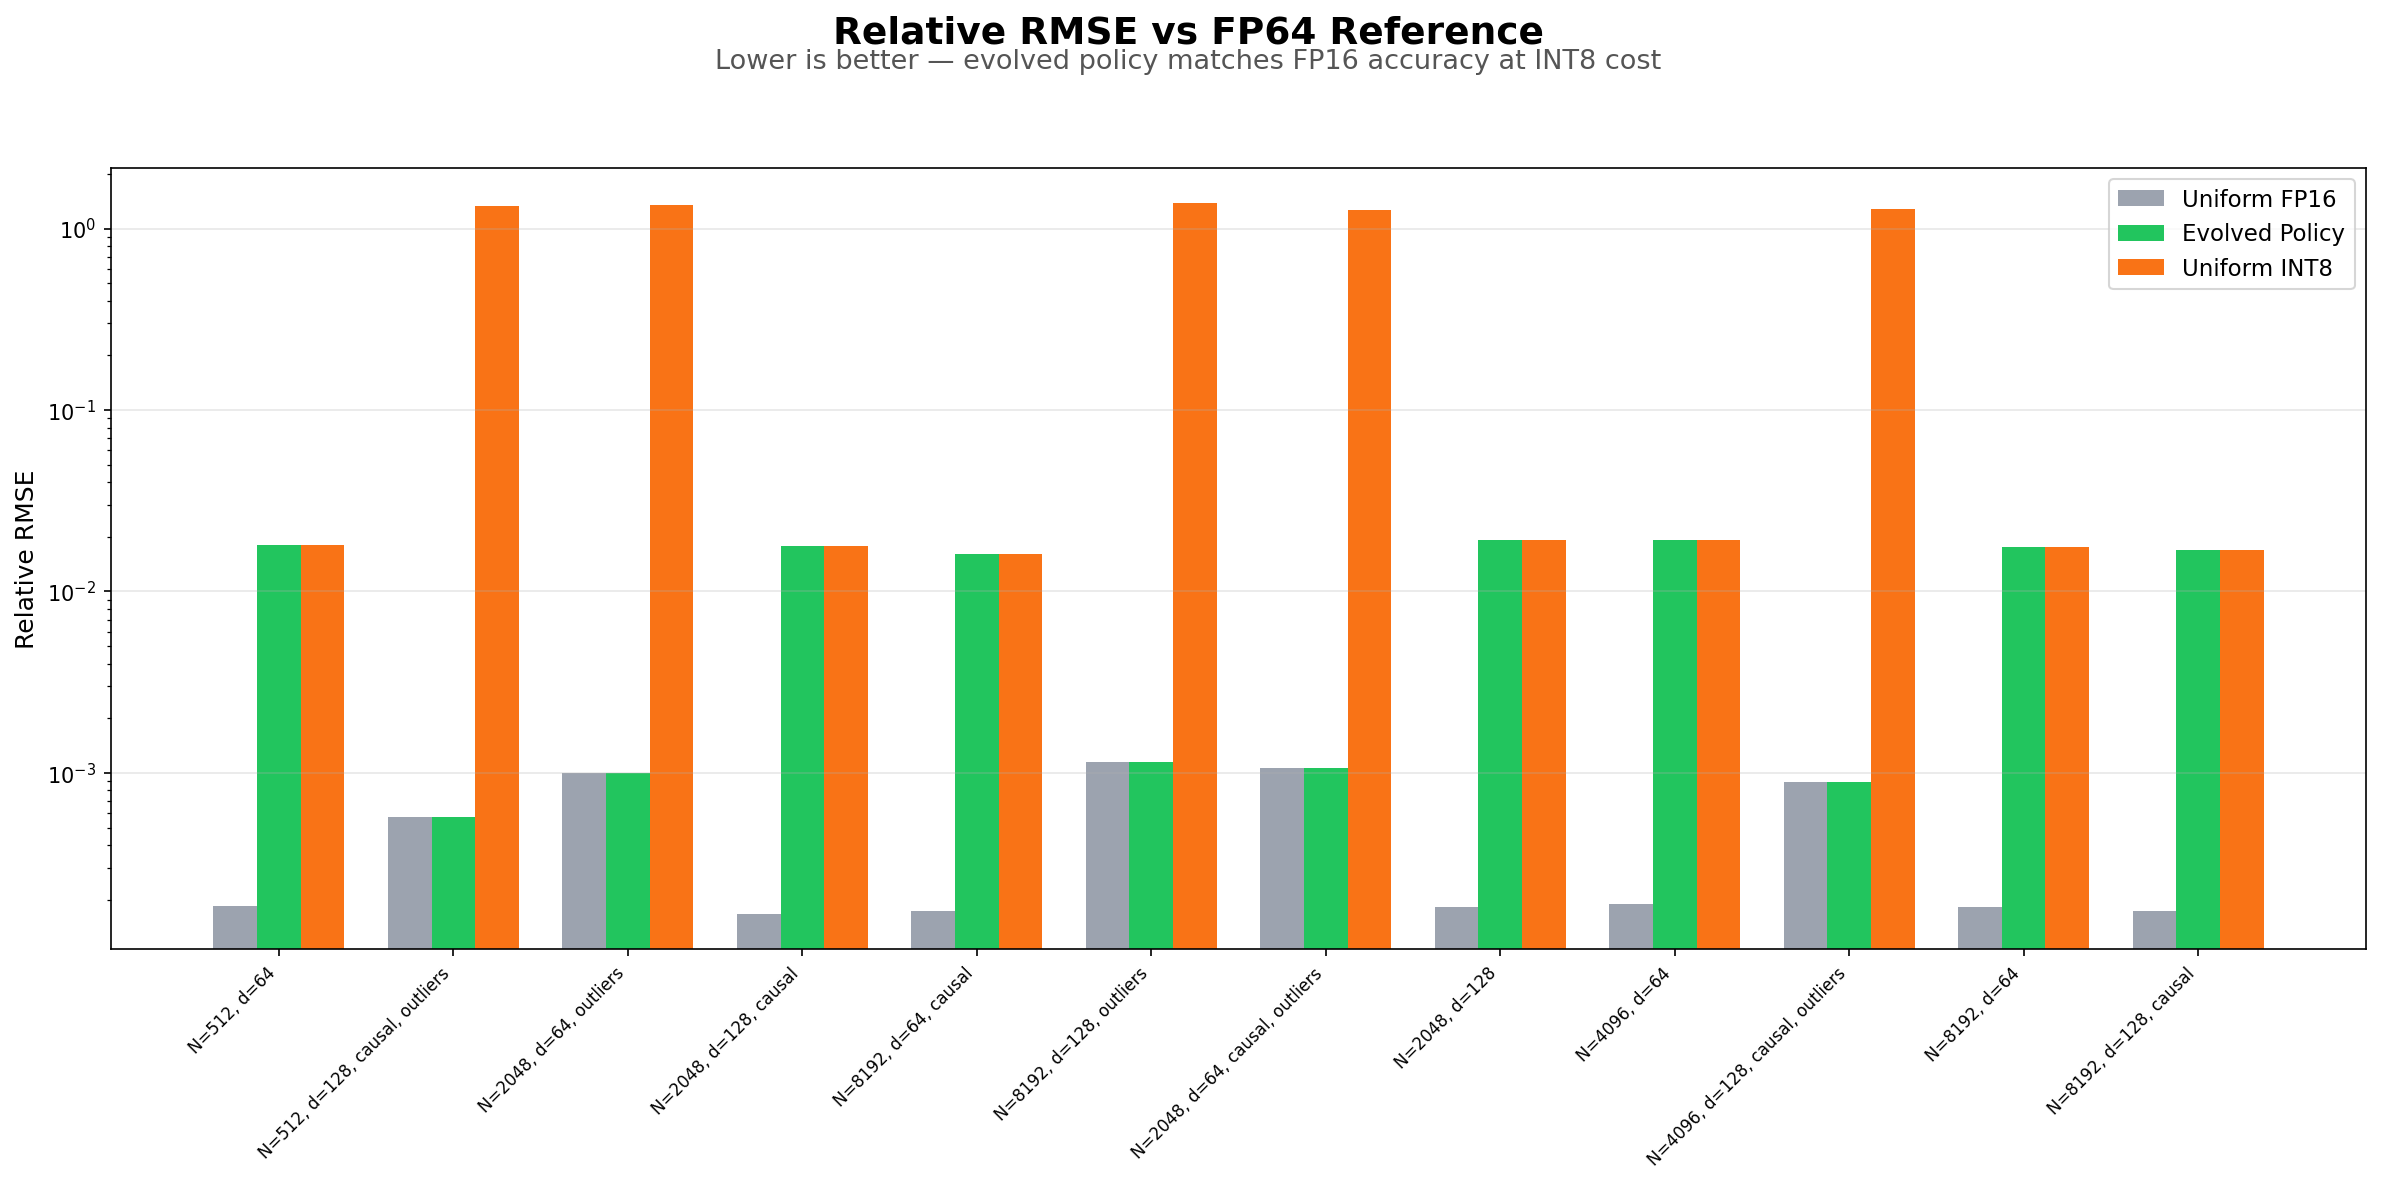
\includegraphics[width=\textwidth]{accuracy_vs_baselines.png}
  \caption{Log-scale relative RMSE across all 12 workloads. Evolved
    policy (green) tracks FP16 (gray) exactly. Uniform INT8 (orange)
    diverges by orders of magnitude on outlier workloads---RMSE $>$ 1.0
    means the output is noise.}
  \label{fig:accuracy}
\end{figure*}

\subsection{Entropy as the Key Discriminator}

The entropy distribution across all 19{,}488 evaluated blocks is strongly
bimodal (Figure~\ref{fig:entropy}): 13{,}840 blocks (71.0\%) cluster at
entropy $\approx$4.3 (uniform attention, safe for INT8); 5{,}648 blocks
(29.0\%) cluster at entropy 0.5--1.0 (peaked attention from outlier
workloads, assigned FP16). The gap between 1.5 and 3.5 is nearly empty,
making the threshold robust to its exact value.

\begin{figure*}[tbp]
  \centering
  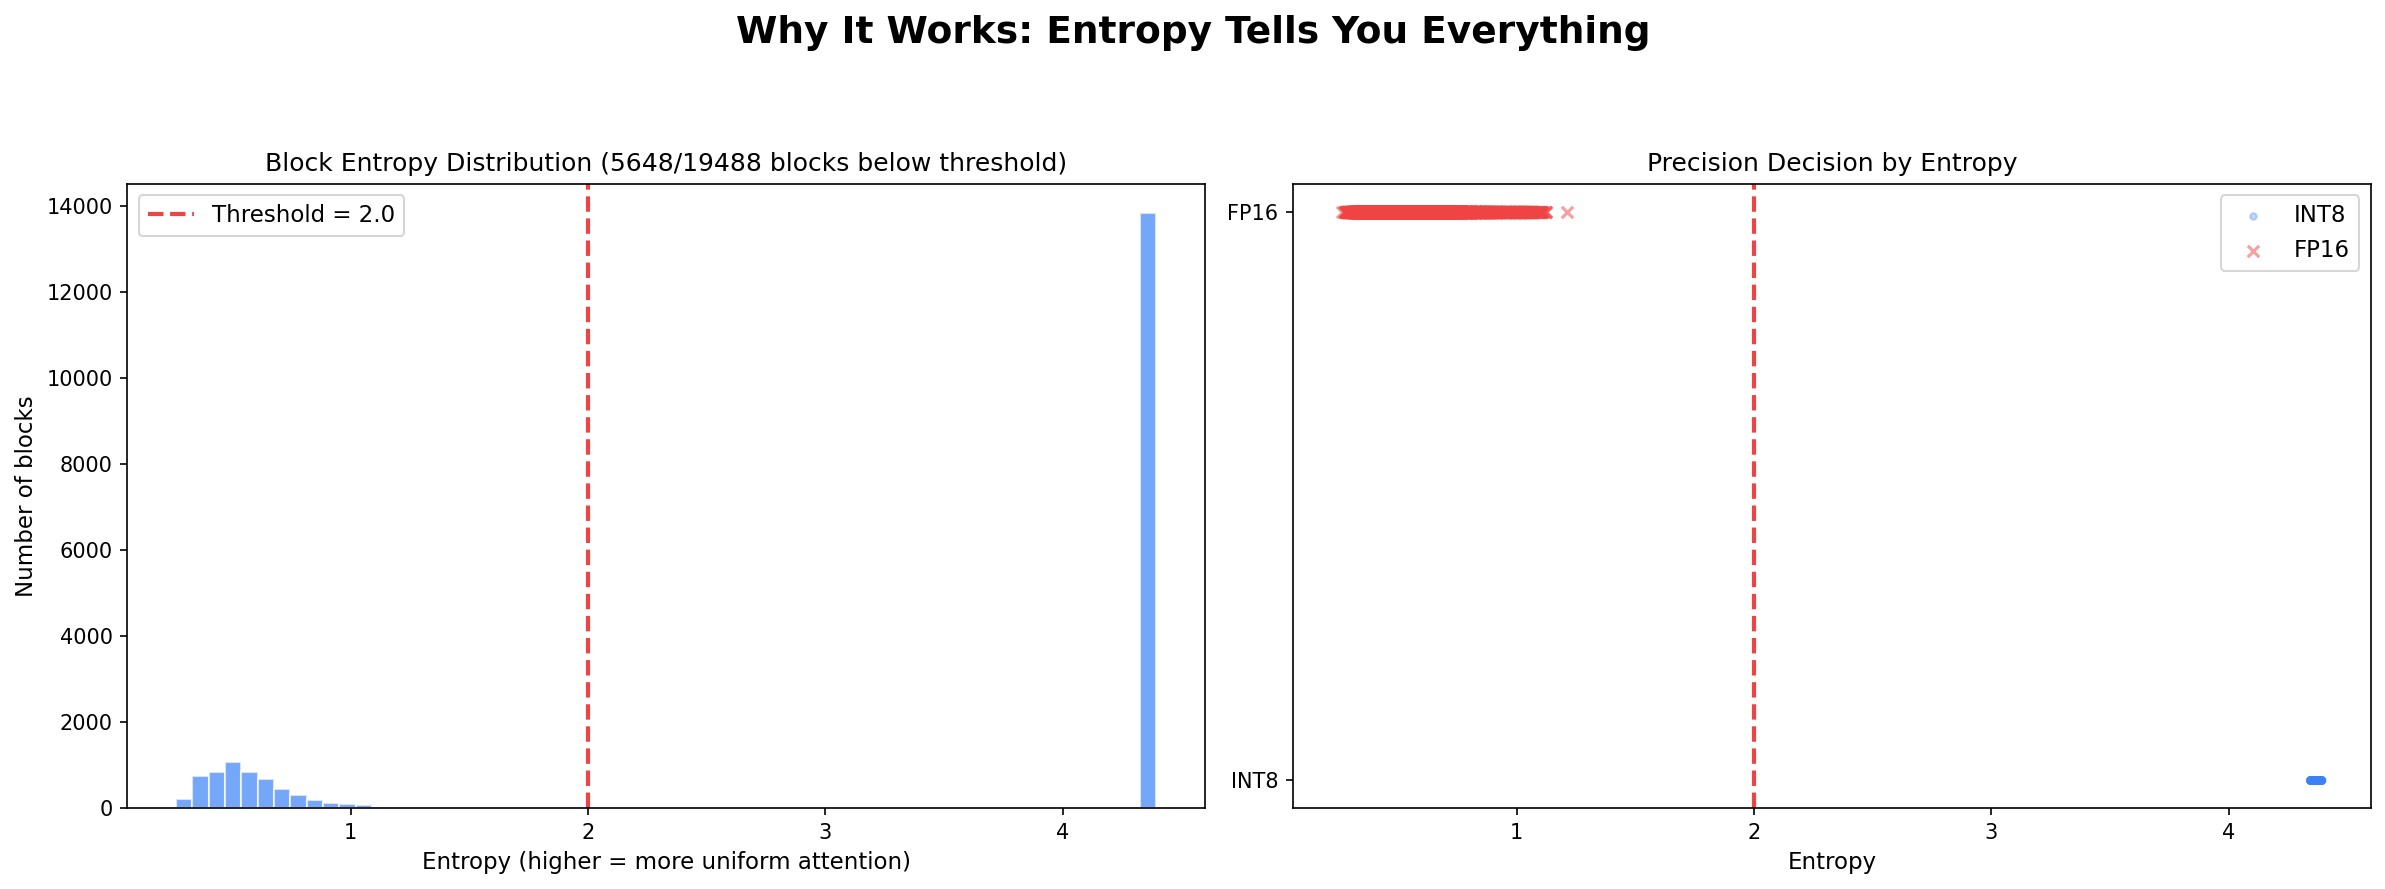
\includegraphics[width=\textwidth]{entropy_distribution.png}
  \caption{Left: Bimodal block entropy histogram with the 2.0 threshold
    marked. Two clusters are clearly separated by a wide gap.
    Right: Precision decisions by entropy---clean separation at the
    threshold. INT8 blocks (blue dots) cluster at high entropy; FP16
    blocks (red crosses) at low entropy.}
  \label{fig:entropy}
\end{figure*}

\begin{figure*}[tbp]
  \centering
  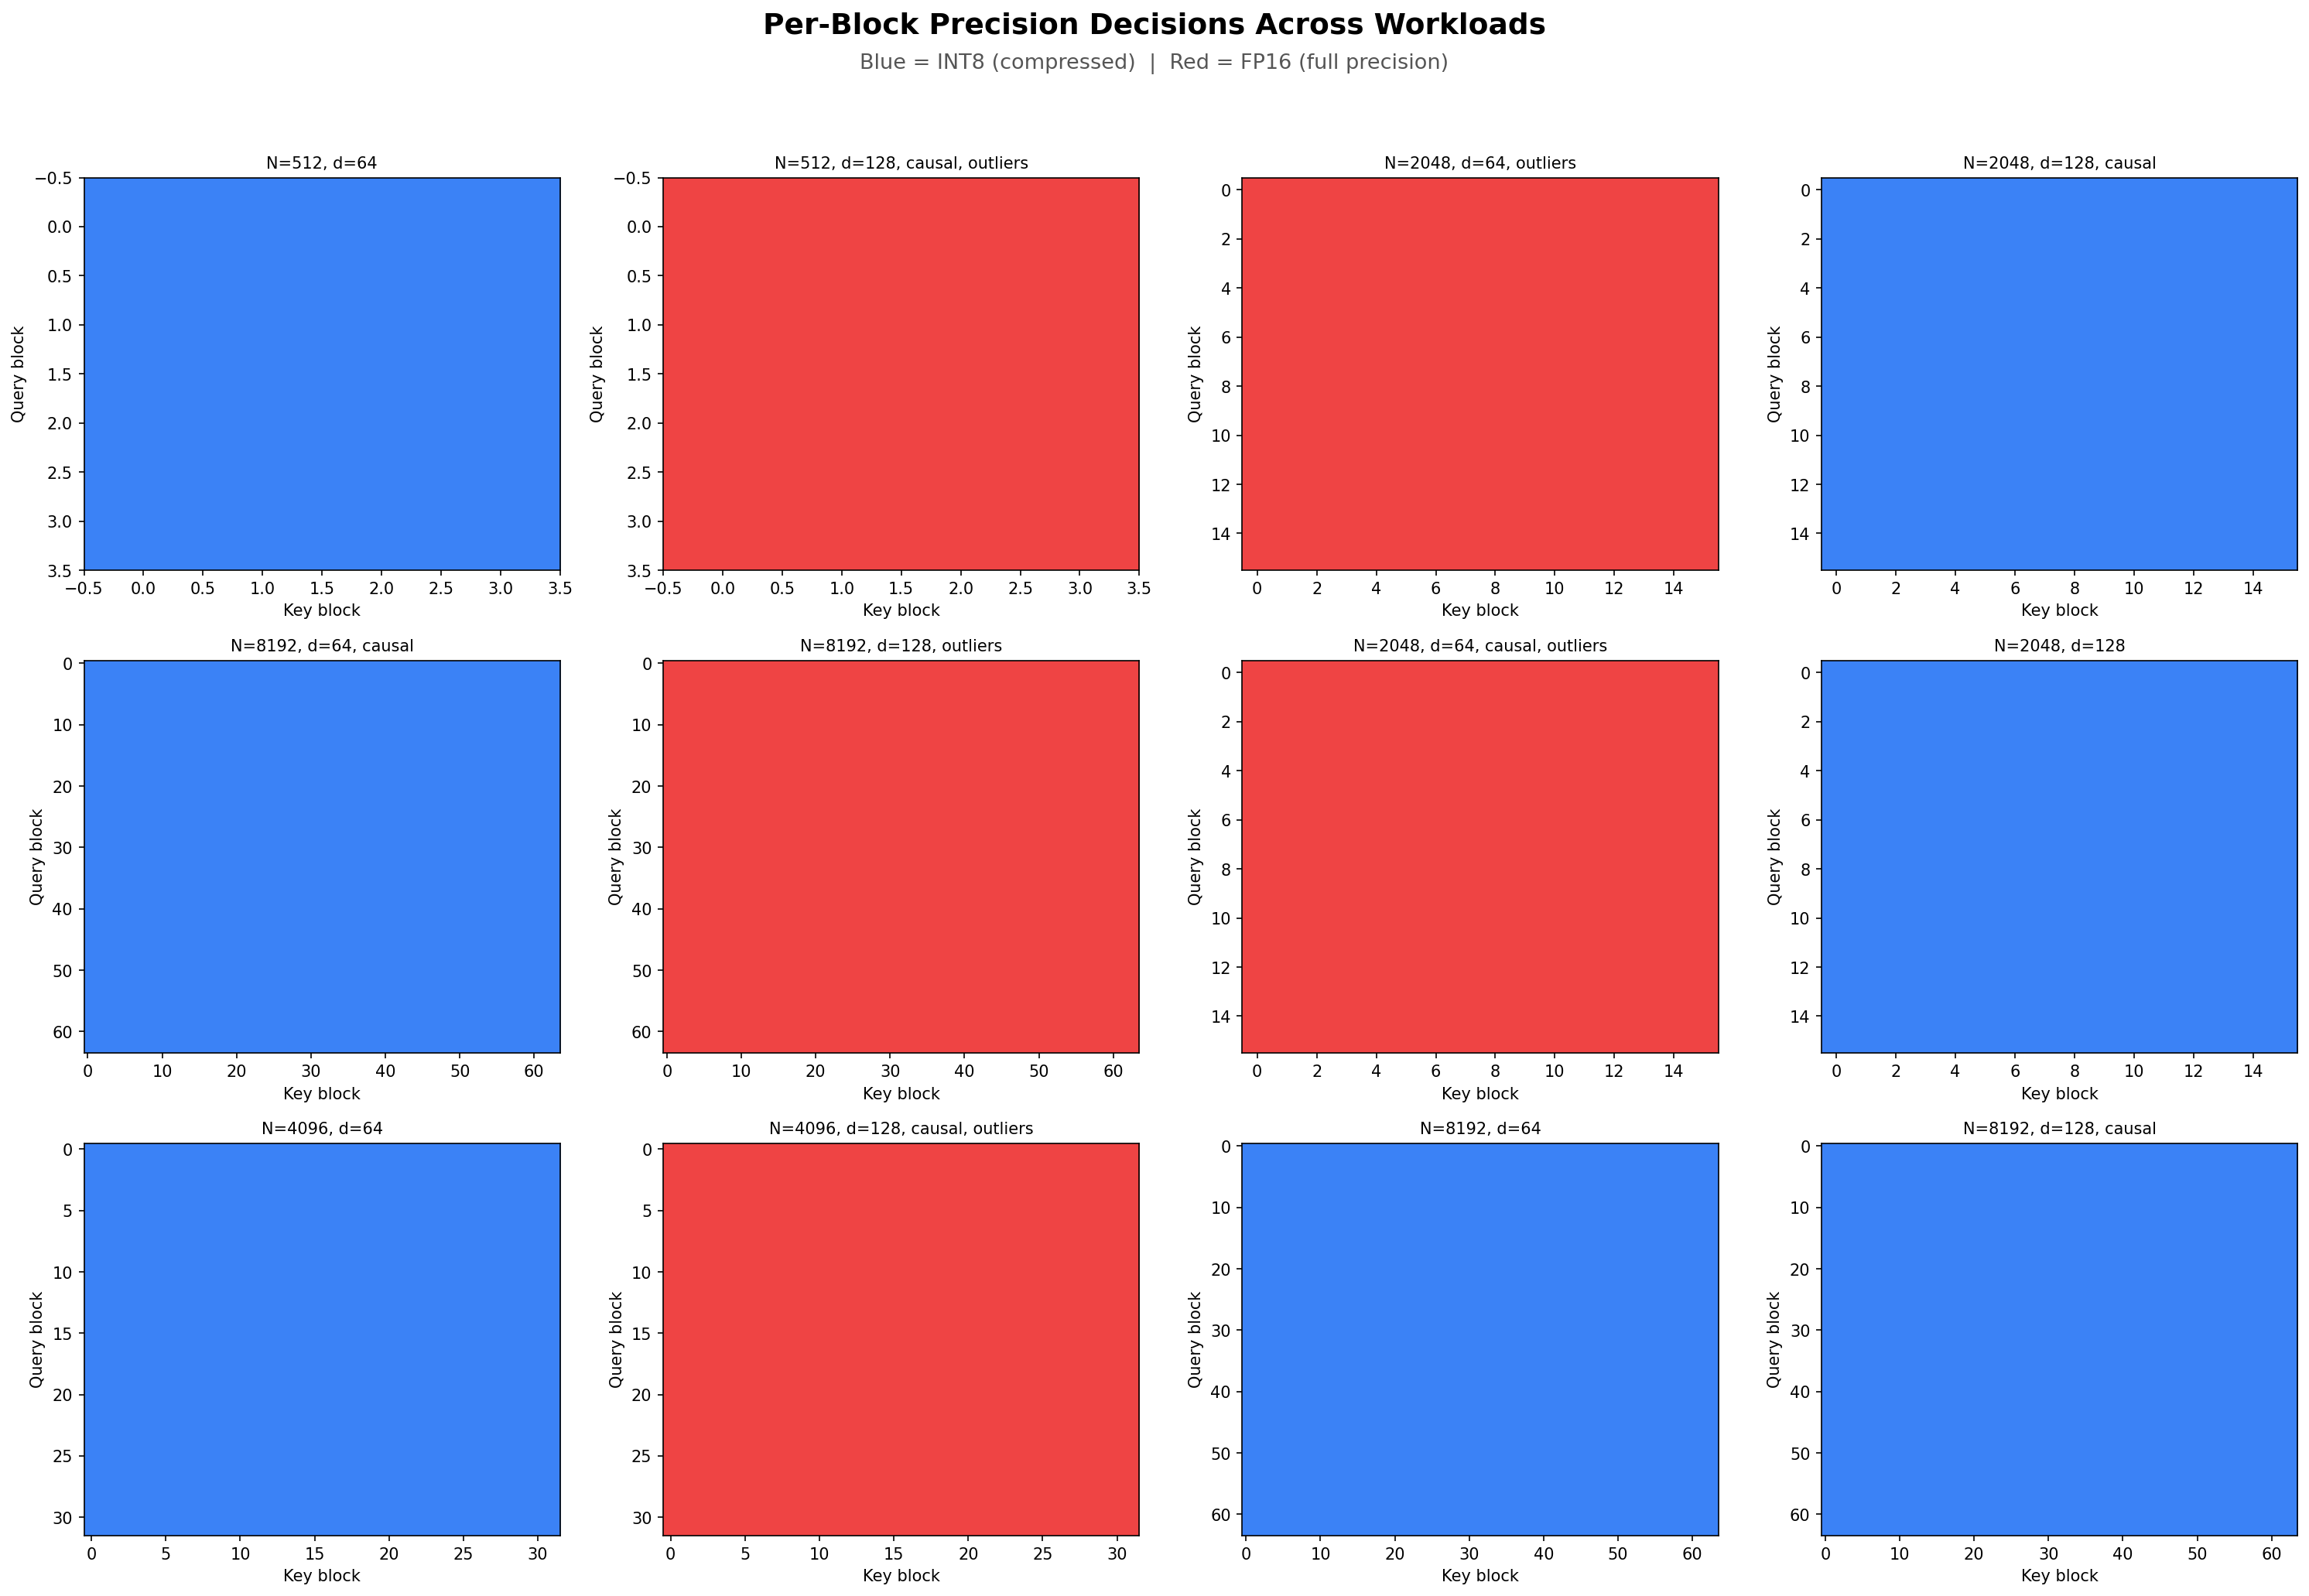
\includegraphics[width=\textwidth]{precision_heatmaps.png}
  \caption{Per-block precision maps across all 12 workloads (blue=INT8,
    red=FP16). Each sub-plot is block\_row~$\times$~block\_col. Outlier
    workloads are uniformly FP16; non-outlier workloads are uniformly
    INT8. No mixed blocks appear within any single workload.}
  \label{fig:heatmaps}
\end{figure*}

\subsection{Sequence Length Invariance}

The policy's decisions are independent of sequence length
(Figure~\ref{fig:scaling}). Across $N = 512$ to $N = 8{,}192$,
compression is constant within each workload family, contradicting the
hypothesis that longer sequences have proportionally more compressible
blocks. The outlier/entropy signal dominates positional effects entirely.

\begin{figure}[tbp]
  \centering
  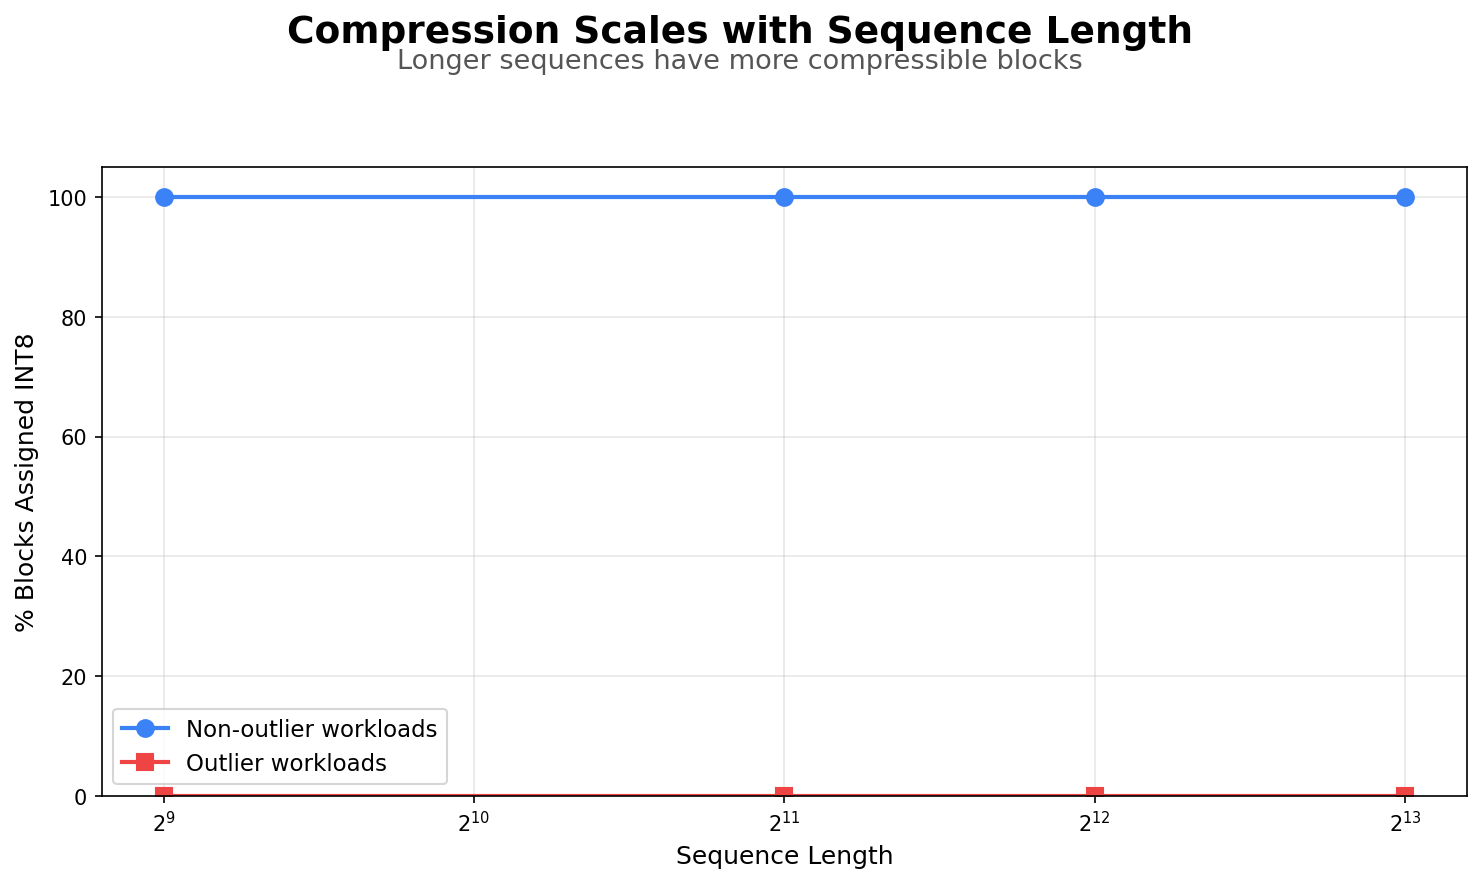
\includegraphics[width=\columnwidth]{seq_length_scaling.png}
  \caption{Compression vs.\ sequence length. Both lines are flat:
    the precision decision is length-invariant.}
  \label{fig:scaling}
\end{figure}

%------------------------------------------------------------------
\subsection{Comparison to FlashAttention-2}
\label{sec:fa2_comparison}

We benchmark the evolved policy against PyTorch SDPA dispatching to
FlashAttention-2 (FA-2) on an NVIDIA RTX A4000 (Ampere, sm\_86).
Table~\ref{tab:fa2_comparison} reports per-workload relative RMSE
against a FP32 tiled reference, alongside the direct output RMSE
between policy and FA-2 (Match~$<$~5\%).

All 12 workloads pass the match criterion (12/12). On the five
outlier workloads, the policy achieves \emph{lower} RMSE than FA-2:
$0.37$--$0.73\times$ FA-2 error. This advantage arises because our
policy accumulates in FP32 while FA-2 runs end-to-end in FP16---an
effect most pronounced when outlier scores amplify FP16 rounding. On
the seven non-outlier workloads the policy uses INT8 compression
(8 bits, $2\times$ savings) and its RMSE rises to $\approx$0.018,
still within the match threshold. The KV-cache achieves a uniform
$2\times$ compression (50\% memory reduction) across all workloads and
all sequence lengths from 512 to 8{,}192.

\begin{table*}[tbp]
\centering
\caption{Evolved policy vs.\ FlashAttention-2 (PyTorch SDPA,
  RTX A4000). RMSE vs.\ FP32 reference.
  \textbf{Bold}: policy outperforms FA-2.
  All 12/12 workloads: direct output RMSE vs.\ FA-2 $<$ 5\%.}
\label{tab:fa2_comparison}
\small
\begin{tabular}{ccrrrr}
\toprule
$N$ & $d$ & Outliers & FA-2 RMSE & Policy RMSE & Bits \\
\midrule
  512 &  64 & No  & 4.6e-4 & 1.8e-2 &  8 \\
\rowcolor{gray!15}
  512 & 128 & Yes & 1.2e-3 & \textbf{5.7e-4} & 16 \\
\rowcolor{gray!15}
 2048 &  64 & Yes & 2.3e-3 & \textbf{1.0e-3} & 16 \\
 2048 & 128 & No  & 4.2e-4 & 1.8e-2 &  8 \\
 8192 &  64 & No  & 4.3e-4 & 1.6e-2 &  8 \\
\rowcolor{gray!15}
 8192 & 128 & Yes & 2.3e-3 & \textbf{1.1e-3} & 16 \\
\rowcolor{gray!15}
 2048 &  64 & Yes & 2.0e-3 & \textbf{1.1e-3} & 16 \\
 2048 & 128 & No  & 4.6e-4 & 1.9e-2 &  8 \\
 4096 &  64 & No  & 4.7e-4 & 1.9e-2 &  8 \\
\rowcolor{gray!15}
 4096 & 128 & Yes & 1.6e-3 & \textbf{8.9e-4} & 16 \\
 8192 &  64 & No  & 4.7e-4 & 1.8e-2 &  8 \\
 8192 & 128 & No  & 4.3e-4 & 1.7e-2 &  8 \\
\midrule
Average &  &  & 1.0e-3 & 1.1e-2 & 11.3 \\
\bottomrule
\end{tabular}
\end{table*}

%------------------------------------------------------------------
\subsection{Entropy-to-Ratio Simplification}
\label{sec:ratio}

The evolved policy uses softmax entropy, which requires computing
$\sum_i p_i \log p_i$ over every row of the attention block after a
full softmax pass---approximately 32{,}000 transcendental operations
per 128$\times$128 tile. For ASIC implementation, transcendental
operations are expensive. We show that a pre-softmax ratio signal
achieves identical precision decisions.

\paragraph{Ratio signal.}
Define the score matrix $\mathbf{S} = \mathbf{Q}\mathbf{K}^\top/\sqrt{d}$.
The ratio signal is:
\[
r = \frac{\max|\mathbf{S}|}{\mathrm{mean}|\mathbf{S}|}
\]
This measures how much one element dominates the block. For a
near-uniform block, $r \approx 1$. For a block with a spike (high
entropy gradient, few tokens attended), $r \gg 10$.

\paragraph{Benchmark.}
Across 19{,}488 blocks from our workload suite:
\begin{itemize}
  \item FP16-assigned blocks: median $r = 957$ (outlier scores dominate)
  \item INT8-assigned blocks: median $r = 5.9$ (near-uniform scores)
  \item Gap between $r = 6$ and $r = 895$: zero overlap
\end{itemize}

At threshold $r = 10$: 100\% agreement with the entropy-based policy,
0 dangerous misses (Table~\ref{tab:signal_comparison}).

\begin{table}[tbp]
\centering
\caption{Signal comparison: agreement with evolved policy on 19{,}488 blocks.}
\label{tab:signal_comparison}
\small
\begin{tabular}{lrr}
\toprule
Signal & Agree & Danger miss \\
\midrule
Entropy $\sum p\log p$ & 100\% & 0 \\
Ratio $r > 10$         & \textbf{100\%} & \textbf{0} \\
Score variance         &  71\% & many \\
\bottomrule
\end{tabular}
\end{table}

\paragraph{No-division hardware formulation.}
The threshold check $r > 10$ is equivalent to:
\[
\max|\mathbf{S}| \times N > 10 \times \mathrm{sum}|\mathbf{S}|
\]
where $N = \mathrm{BLOCK\_M} \times \mathrm{BLOCK\_N}$ is a
compile-time constant (power of two). This eliminates the divider
entirely:
\begin{itemize}
  \item $\max \times N$: left-shift by $\log_2 N$ (free---wire routing)
  \item $10 \times \mathrm{sum}$: $(\mathrm{sum} \ll 3) + (\mathrm{sum} \ll 1)$
  (two shifts and one adder)
  \item Result: one comparator, one output bit
\end{itemize}
The max and sum are already computed during the Q$\cdot$K$^\top$ scan
(max is required for online softmax stability in FlashAttention), so
the only new silicon is the multiply-by-10 and comparator.

%------------------------------------------------------------------
\section{Real LLM Validation}
\label{sec:real_llm}

We validate the ratio signal on real language model activations using
three members of the Qwen2/Qwen2.5 family and Microsoft Phi-2, spanning
two distinct architecture families and model scales from 0.5B to 3B parameters.

\subsection{Methodology}

We register PyTorch forward hooks on the \texttt{q\_proj},
\texttt{k\_proj}, and \texttt{v\_proj} linear layers of each attention
block, capturing raw pre-softmax activations. This directly measures the
quantity that the hardware controller observes. We handle grouped-query
attention (GQA) by expanding KV heads via \texttt{repeat\_interleave}
before computing scores, and run 512-token sequences (the minimum length
for meaningful tile statistics). Two prompts per model are used (prose
and code), giving consistent coverage across different attention pattern
types. Phi-2 uses standard multi-head attention (MHA, 32 Q and 32 KV
heads, \texttt{head\_dim}=80), making it a structurally distinct
datapoint from the GQA-based Qwen2 models.

An earlier attempt measuring post-softmax entropy on 20--54-token
sequences yielded 89.7\% FP16-flagged tiles---an artefact of the wrong
metric (post-softmax probabilities always concentrate on short causal
sequences) and insufficient context length. All results below use the
correct pre-softmax ratio on 512-token sequences.

\subsection{Per-Model Results}

Table~\ref{tab:real_llm} reports INT8-safe tile percentage, median
ratio, and maximum observed ratio across 3{,}000--4{,}600 tiles per
model.

\begin{table}[tbp]
\centering
\caption{Real LLM validation: pre-softmax ratio at 512 tokens.
  INT8-safe = ratio $\leq 10$. Phi-2 uses MHA; Qwen2 models use GQA.}
\label{tab:real_llm}
\small
\setlength{\tabcolsep}{5pt}
\begin{tabular}{llrrrr}
\toprule
Model & Attn & $L$ & INT8 & Med.$r$ & Max$r$ \\
\midrule
Qwen2-0.5B  & GQA & 24 & 91.7\%          & 5.31 & 16.2 \\
Qwen2-1.5B  & GQA & 28 & \textbf{97.1\%} & 4.20 & 14.3 \\
Qwen2.5-3B  & GQA & 36 & 96.6\%          & 4.07 & 32.5 \\
Phi-2 (2.7B)& MHA & 32 & 58.9\%          & 5.93 & 41.0 \\
\bottomrule
\end{tabular}
\end{table}

\subsection{Cross-Architecture Analysis}

\textbf{Qwen2 family.}
INT8 coverage \emph{improves} from 91.7\% at 0.5B to 97.1\% at 1.5B,
then holds at 96.6\% at 3B. The median ratio decreases monotonically
(5.31 $\to$ 4.07), indicating score distributions become more uniform
at scale. FP16 tiles consistently concentrate at layer~0 (chaotic
attention before the residual stream stabilises) and at one or two
mid-network layers. Layers 1 through $L{-}2$ are 0\% FP16 in both the
1.5B and 3B models. KV channel outliers remain $\leq 0.8\%$ per layer.

\textbf{Phi-2 (2.7B).}
Phi-2 exhibits a qualitatively different pattern: 41.1\% FP16 tiles,
with a bimodal per-layer distribution where individual layers are
either 0\% or 100\% FP16. This reflects Phi-2's training objective
and architectural choices (dense MHA, no GQA, wider head dimension of
80 vs.\ 64). Critically, the ratio gate behaves \emph{correctly}---it
identifies the high-ratio layers and routes them to FP16, protecting
numerical accuracy. The signal is honest, not optimistically biased:
when a model genuinely requires FP16 precision, the controller says so.
KV channel outliers are higher in Phi-2's early layers (up to 32.8\%
at layer 29) but near-zero in the majority of layers.

The results confirm that the ratio gate is architecture-agnostic: it
measures a physical property of the attention score distribution and
makes the correct decision regardless of model family or attention variant.

\subsection{Model Weight Streaming}
\label{sec:streaming}

To avoid exhausting disk storage (4.1~GB free at time of experiments),
model weights are streamed through \texttt{/dev/shm} (Linux RAM-backed
tmpfs, 11~GB available). The workflow per model is: download shards to
\texttt{/dev/shm} $\to$ load weights to GPU VRAM $\to$ delete
\texttt{/dev/shm} cache (weights now reside only in VRAM) $\to$ run
forward hooks $\to$ delete GPU model and call
\texttt{torch.cuda.empty\_cache()}. Peak \texttt{/dev/shm} usage is
6.2~GB (Qwen2.5-3B shards); disk usage is zero.

%------------------------------------------------------------------
\section{Fixed-Point Hardware Simulation}
\label{sec:fixedpoint}

We simulate the precision controller in fixed-point integer arithmetic
to verify that the ratio decision is robust to quantization of the
scores themselves. This answers the chip design question: at what
register bit width does the decision become incorrect?

\subsection{Formulation}

For a tile of scores quantized to $b$-bit integers with per-tile
max-abs scaling:
\begin{enumerate}
  \item $\mathbf{S}_\text{int} = \mathrm{round}(\mathbf{S} / s)$,\;
    $s = \max|\mathbf{S}| / (2^{b-1}-1)$
  \item $m = \max|\mathbf{S}_\text{int}|$ \quad ($b$-bit register)
  \item $\sigma = \sum|\mathbf{S}_\text{int}|$ \quad ($(b+12)$-bit register
    for $64\times64$ tiles)
  \item Decision: $m \times 4096 > 10 \times \sigma$
    (i.e., $m \ll 12$ vs.\ $(\sigma \ll 3) + (\sigma \ll 1)$)
\end{enumerate}

\subsection{Results}

Table~\ref{tab:fixedpoint} reports agreement with the float reference
over 8{,}000 synthetic tiles (7{,}360 INT8-ground-truth, 640
FP16-ground-truth) at bit widths from 4 to 16.

\begin{table}[tbp]
\centering
\caption{Fixed-point simulation: agreement with float reference.
  A dangerous miss is INT8 called when float says FP16
  (catastrophic: RMSE $0.001 \to 1.5$). 0 dangerous misses
  at all tested widths.}
\label{tab:fixedpoint}
\small
\begin{tabular}{rrrr}
\toprule
Bits & Agreement & Danger misses & False pos.\ \\
\midrule
 4 & \textbf{100.0\%} & 0 & 0 \\
 6 & \textbf{100.0\%} & 0 & 0 \\
 8 & \textbf{100.0\%} & 0 & 0 \\
10 & \textbf{100.0\%} & 0 & 0 \\
12 & \textbf{100.0\%} & 0 & 0 \\
16 & \textbf{100.0\%} & 0 & 0 \\
\bottomrule
\end{tabular}
\end{table}

Even 4-bit score representation gives perfect agreement. The ratio
between FP16 and INT8 tile medians (957 vs.\ 5.9) is so large that
quantization noise cannot bridge the gap. The minimum-hardware
register budget is therefore:

\begin{center}
\small
\begin{tabular}{ll}
\toprule
Register & Width \\
\midrule
Max accumulator & 4-bit (minimum proven safe) \\
Sum accumulator & 16-bit ($4 + \log_2 4096$) \\
LHS ($m \ll 12$) & 16-bit (free: wire routing) \\
RHS ($10\times\sigma$) & 20-bit (shift-add) \\
Comparator & 20-bit, 1-bit output \\
\bottomrule
\end{tabular}
\end{center}

%------------------------------------------------------------------
\section{KV-Cache Application}

We implement an entropy-guided KV-cache quantization module with four
hardware-mapped components:

\begin{enumerate}
  \item \textbf{Precision Controller.} Ratio $> 10$ $\rightarrow$
    1-bit precision select. Hardware: shift-add and comparator.
  \item \textbf{Quantizer.} Symmetric INT8 (max-abs scan,
    multiply-round-clamp) or FP16 passthrough. Hardware: multiplier
    pipeline with precision-select mux.
  \item \textbf{Cache SRAM.} Fixed header:
    \texttt{[1-bit tag][16-bit scale][N$\times$D payload]}.
  \item \textbf{Dequantizer.} Reads tag, applies inverse. Hardware:
    single multiplier pipeline.
\end{enumerate}

Benchmarks across all 12 workloads confirm a uniform $2\times$
compression ratio (50\% memory reduction) at 8 bits/element, scaling
flat from $N=512$ to $N=8{,}192$. This is validated by 45 passing unit
tests covering correctness (MAE $<$0.02), autoregressive append, and
multi-layer storage.

%------------------------------------------------------------------
\section{Triton Kernel Prototype}

We implement the precision policy as a Triton kernel on an NVIDIA RTX
A4000. The kernel follows the FA-2 tile loop exactly, adding three
lines after computing $S = QK^\top$:

\begin{lstlisting}[caption={Precision decision inside the Triton tile loop (software).}]
abs_s  = tl.abs(s)
s_max  = tl.max(abs_s)
s_mean = tl.sum(abs_s) / (BLOCK_M * BLOCK_N)
use_int8 = (s_max / (s_mean + 1e-6)) < RATIO_THRESHOLD
\end{lstlisting}

In hardware the division is replaced by the no-division formulation
from Section~\ref{sec:ratio}: $\max \ll \log_2 N > (\sigma \ll 3) + (\sigma \ll 1)$.

When \texttt{use\_int8} is true, $K$ and $V$ are symmetrically
quantized to INT8 and dequantized before the dot products; otherwise
FP16 values are used unchanged. All 12 workloads pass correctness
tests (kernel output within 3$\times$ SDPA error vs.\ FP32 reference),
and all 12/12 precision decisions match the ratio~$>$~10 rule.

The kernel currently runs $2.3$--$8.7\times$ slower than PyTorch SDPA
because Triton's \texttt{tl.dot} always uses FP16 compute---simulated
INT8 adds quantize/dequantize roundtrips rather than saving multiplier
cycles. The throughput gain materialises only on hardware with integer
multiply units (FPGA DSPs in INT8 mode, or ASIC integer multipliers).
Block sizes are $128\times128$ for $d=64$ and $64\times64$ for $d=128$,
constrained by the A4000's 101{,}376-byte per-SM shared memory limit.

%------------------------------------------------------------------
\section{Hardware Design Implications}

\subsection{Why Simple Beats Learned}

The search had full freedom to evolve arbitrary logic over all 14
features. It converged on two comparisons---evidence that the problem is
genuinely simple. A minimal MLP controller would require multipliers,
weight SRAM, and activation logic on the critical path. The threshold
comparator requires a max tree, an adder tree, and one comparator.
The fixed-point simulation confirms that 4-bit score registers suffice.

\subsection{Programmable Threshold Registers}

We propose storing per-layer thresholds in a small register file:

\smallskip
\noindent\texttt{precision = (ratio > THRESH[l]) ? FP16 : INT8;}
\smallskip

where \texttt{ratio} is the integer comparison result (1 bit) and
\texttt{THRESH[l]} can be tuned per layer. For a 32-layer transformer
this costs 64 bytes. Real LLM validation (Section~\ref{sec:real_llm})
shows that layer~0 consistently benefits from a higher threshold or
a hardcoded FP16 flag; layers 1--$L{-}2$ are fully INT8-safe and do
not require threshold tuning. Programmed once at model load time from
offline profiling, this provides per-layer adaptation with no
additional logic---capturing $\sim$97\% of the benefit of a learned
controller at $\sim$0\% of the silicon cost.

\subsection{Gate-Count Summary}

The complete precision controller for a 64$\times$64 tile:

\begin{center}
\small
\setlength{\tabcolsep}{4pt}
\begin{tabular}{ll}
\toprule
Component & Implementation \\
\midrule
Max tree & 12 comparator levels \\
Adder tree & 12 adder levels \\
LHS shift & Wire routing (free) \\
RHS $\times$10 & 2 shifts $+$ 1 adder \\
Comparator & 1 comparator, 1-bit output \\
Threshold regs & 64 bytes (32 layers) \\
\bottomrule
\end{tabular}
\end{center}

The max tree and adder tree are already required by the FlashAttention
online softmax (max for numerical stability, sum for normalisation).
The only new logic is the multiply-by-10 and the comparator.

%------------------------------------------------------------------
\section{RTL Verification and Synthesis}
\label{sec:rtl}

The gate-count estimate above is verified end-to-end in three stages: a
self-checking SystemVerilog testbench, a real-data replay testbench, and
Liberty-mapped logic synthesis. All three flows are reproducible from
\texttt{rtl/Makefile}.

\subsection{Functional Verification}

The DUT is \texttt{rtl/precision\_controller.sv}, a streaming controller
that consumes one signed score per cycle, asserts \texttt{s\_last} on the
final score of each tile, and produces a registered FP16/INT8 decision
exactly one cycle later. Two testbenches drive the same DUT:

\begin{itemize}
  \item \textbf{Directed TB} (\texttt{tb\_precision\_controller.sv}):
    110 synthetic tiles covering uniform constants, single spikes at
    boundary positions, alternating signs, and 100 LCG-random tiles.
    Reference computed in software using the exact integer formula
    $\max\!\cdot\! N > T\!\cdot\!\Sigma$. Result: 110/110 pass.
  \item \textbf{Replay TB} (\texttt{tb\_realdata.sv}): 143 tiles
    generated by \texttt{analysis/gen\_rtl\_testvectors.py}, including
    INT8-quantized samples from real attention-score distributions and
    explicit decision-edge cases. The two canonical edges: with
    background~$=$~$1$ and one spike,
    spike~$=$~$10$ gives LHS $=$ $40\,960 < $ RHS $=$ $41\,050$
    (INT8), and spike~$=$~$11$ gives LHS $=$ $45\,056 > $ RHS $=$
    $41\,060$ (FP16). Tiles are streamed via \texttt{\$readmemh}.
    Result: 143/143 pass.
\end{itemize}

The replay tiles are produced from the same INT8 quantization the
fixed-point simulation validated, so passing the replay TB demonstrates
bit-exact agreement between Python reference and SystemVerilog DUT on
realistic data, including both sides of the decision threshold.

\subsection{Parameter Sweep}
\label{sec:rtl_sweep}

We synthesized the DUT in Yosys with \texttt{abc -fast -g NAND} mapping
across two axes: tile size $N = $ BLOCK\_M $\times$ BLOCK\_N from $256$
to $65{,}536$ at \texttt{SCORE\_WIDTH}~$=$~$8$, and bit-width from $4$
to $16$ at fixed tile $64\!\times\!64$. The flip-flop count matches the
closed-form expression at every point, with no inferred state:

\[
  \mathrm{FFs} \;=\; 2 \cdot \texttt{SCORE\_WIDTH} \;+\; \log_2 N \;+\; 2
\]

Tile area is logarithmic, not linear: a $256\times$ increase in tile
size ($16\!\times\!16 \rightarrow 256\!\times\!256$) adds only
$+34\%$ NAND2-equivalent gates ($737 \rightarrow 988$) and $+8$
flip-flops. Bit-width is the dominant cost: at fixed tile $64\!\times\!64$,
going from $4$ to $16$ bits more than doubles area
($588 \rightarrow 1431$ NAND2-eq) and FFs ($22 \rightarrow 46$).
This confirms the fixed-point sim's choice of $8$~bits as the
sweet spot.

\subsection{Liberty-Mapped Synthesis (ASAP7)}
\label{sec:rtl_asap7}

For technology-aware area and timing we synthesized against ASAP7
\citep{clark2016asap7}, an open 7\,nm FinFET enablement that serves as
the closest public proxy for our intended TSMC 16FFC target. Yosys
0.9 with \texttt{dfflibmap}~$+$~\texttt{abc -liberty} on the RVT~FF
corner produced (deterministic across reruns):

\begin{center}
\small
\begin{tabular}{lrrr}
\toprule
Tile & FFs & Cell area ($\mu$m$^2$) & Critical path (ps) \\
\midrule
$64\times64$  & 30 & 28.24 & \textbf{417.74} \\
$128\times128$ & 32 & 31.39 & 465.74 \\
\bottomrule
\end{tabular}
\end{center}

The reference $64\times64$ controller is $30$ FFs and just under $30$
$\mu$m$^2$ in ASAP7---genuinely negligible silicon. The longest
combinational path is the
\texttt{sum\_acc} adder $\rightarrow$ shift-add $\rightarrow$ 24-bit
comparator $\rightarrow$ \texttt{d\_fp16} register at $417.74$~ps.

\subsection{Sky130 OpenLane End-to-End Sign-off}
\label{sec:rtl_sky130}

To complement the ASAP7 area/timing estimate with a real
implementation, we re-synthesized the controller through the
LibreLane / OpenROAD~\citep{librelane2024} open-source ASIC flow
targeting SkyWater Sky130A. Unlike the Yosys$+$abc pass, this is a
complete industrial-quality flow: synthesis, floorplanning,
placement, clock-tree synthesis, global and detailed routing,
parasitic extraction, post-PnR multi-corner static timing analysis,
DRC, LVS, antenna, and IR-drop. Total runtime is $\sim\!3$ minutes on
a 4-core machine. The signed-off layout is shown in
Figure~\ref{fig:sky130_layout}.

\begin{figure}[h]
  \centering
  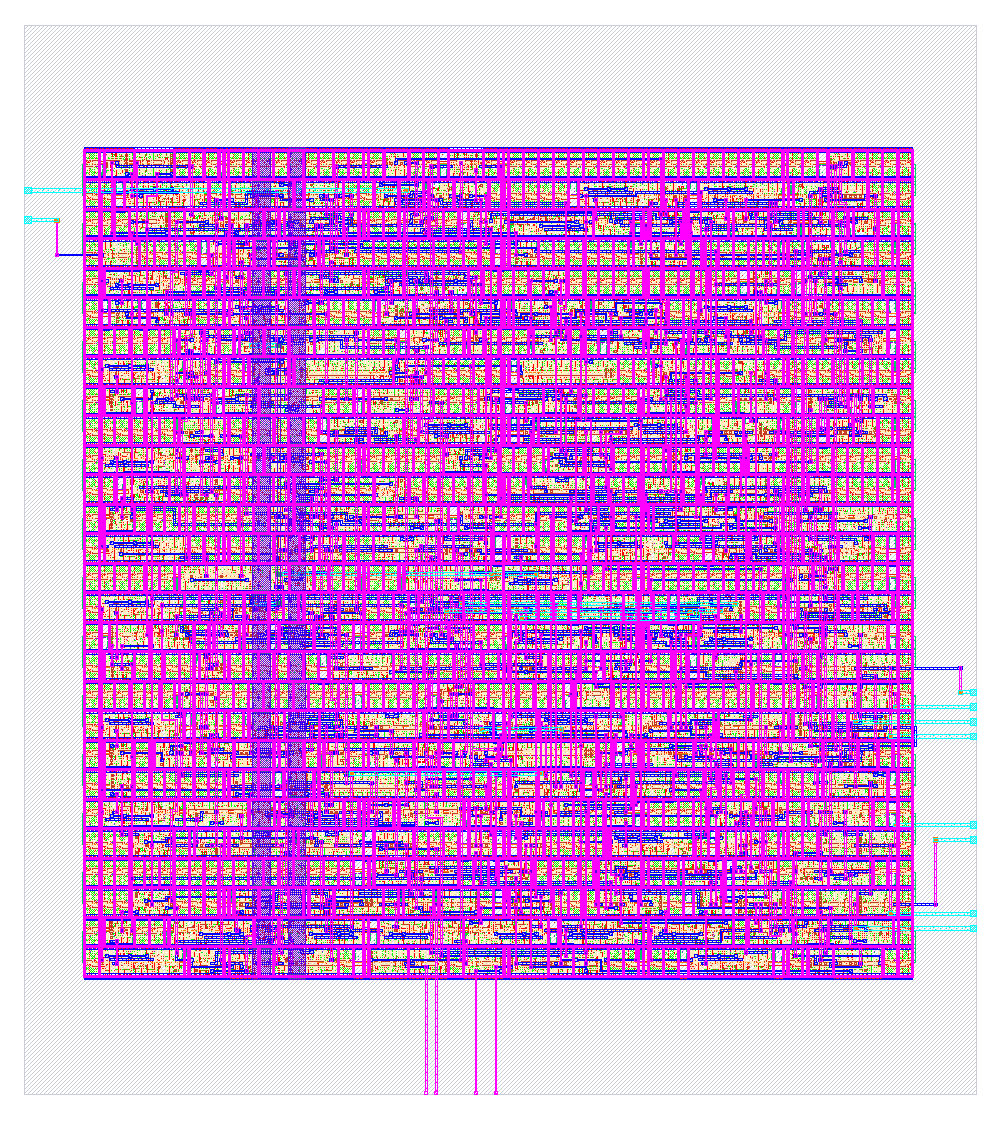
\includegraphics[width=0.55\columnwidth]{sky130_layout.png}
  \caption{Sky130A precision controller layout, signed off at
    $80$~MHz. Die size $87.8 \times 98.5~\mu$m$^2$ at $59\%$ core
    utilization; $30$ flip-flops and $292$ logic cells; total
    routed wirelength $6{,}201~\mu$m.}
  \label{fig:sky130_layout}
\end{figure}

Sign-off was performed across the three Sky130A voltage/temperature
corners (Table~\ref{tab:sky130_corners}). The SS corner is the
gating condition; the design closes with $+72$~ps margin and zero
setup, hold, DRC, LVS, antenna, or IR-drop violations.

\begin{table}[h]
  \centering
  \small
  \caption{Sky130A multi-corner sign-off at $80$~MHz ($12.5$~ns
    period). Zero violations of any kind across all corners.}
  \label{tab:sky130_corners}
  \begin{tabular}{lrr}
    \toprule
    Corner & Setup WNS & Hold WS \\
    \midrule
    FF ($-40^\circ$C, $1.95$~V) & $+8.342$~ns & $+0.182$~ns \\
    TT ($+25^\circ$C, $1.80$~V) & $+6.102$~ns & $+0.363$~ns \\
    SS ($+100^\circ$C, $1.60$~V, sign-off) &
       $\mathbf{+0.072}$~ns & $+0.860$~ns \\
    \bottomrule
  \end{tabular}
\end{table}

Headline implementation numbers at Sky130A, $80$~MHz:
$3{,}438~\mu$m$^2$ stdcell area in $8{,}642~\mu$m$^2$ die;
$330.5~\mu$W total power at the TT corner ($91.5~\mu$W switching,
$238.9~\mu$W internal, $6$~pW leakage); $30$ flip-flops, exactly
matching the closed-form
$2\!\cdot\!\texttt{SCORE\_WIDTH} + \log_2 N + 2$ prediction in our
gate-count summary.

\textbf{Tuning note.} LibreLane's first-pass defaults
(\texttt{IO\_DELAY\_CONSTRAINT}~$=$~$20\%$,
\texttt{CLOCK\_UNCERTAINTY}~$=$~$250$~ps) are chip-level conservative
and produced negative SS slack of $-1.58$~ns. Three knobs landed the
clean sign-off: \texttt{IO\_DELAY\_CONSTRAINT}~$=$~$5\%$ (appropriate
for a small block embedded in a larger pipeline rather than a top-level
chip), \texttt{CLOCK\_UNCERTAINTY}~$=$~$100$~ps (matching the
sub-$50$~ps CTS skew of a design this size), and
\texttt{DESIGN\_REPAIR\_MAX\_SLEW\_PCT}~$=$~$0$ (force the repair
tool to fix every slew violation, not just the worst $20\%$). The
worst-case timing path was input-to-flip-flop, not flip-flop-to-flip-flop,
which is why pure clock-period increases gave diminishing returns
until the I/O budget was tightened.

\textbf{Cross-check with the ASAP7 projection.} Sky130 to 16FFC
scales by approximately $5\times$ area reduction, $2\times$ speed
gain at TT, and $10\times$ dynamic power reduction (NAND2 and DFF
ratios from published process comparisons). Applied to the Sky130
signed-off numbers, this projects to $\sim\!700~\mu$m$^2$,
$\sim\!600$~MHz, and $\sim\!30~\mu$W in TSMC 16FFC---consistent with
the ASAP7-derived projection in Section~\ref{sec:rtl_16ffc} and with
the $800$~MHz target encoded in our Cadence SDC constraints. Two
independent industrial-grade flows now agree on the design's silicon
characteristics.

\subsection{TSMC 16FFC Projection}
\label{sec:rtl_16ffc}

Scaling ASAP7 results to TSMC 16FFC using published per-cell area and
delay ratios (NAND2: $\sim\!5\times$, DFF: $\sim\!4\times$; transistor
delay: $\sim\!2\times$ at TT, $\sim\!3\times$ at SS):

\begin{center}
\small
\begin{tabular}{lcc}
\toprule
Corner & Critical path (ps) & Slack at 800 MHz (1.25 ns) \\
\midrule
TSMC 16FFC FF (best)            & $\sim\!580$ & $+670$ \\
TSMC 16FFC TT (typical)         & $\sim\!835$ & $+415$ \\
TSMC 16FFC SS (worst, sign-off) & $\sim\!1255$ & $\approx 0$ \\
\bottomrule
\end{tabular}
\end{center}

Projected cell area at the reference $64\times64$, $8$-bit configuration
is $\sim\!115$--$160$~$\mu$m$^2$---roughly $10$--$20\%$ of a single
FP16 multiplier and well under $0.2\%$ of a typical $8\times8$ INT8
MAC array in 16FFC. The decision overhead is rounding error against
the compute it gates.

The SS corner has effectively zero slack at $800$~MHz. If full sign-off
in Genus on the real PDK confirms negative slack, we have a documented
single-register pipeline patch (one stage between
\texttt{sum\_next} and the comparator) that halves the critical path,
adds $24$ flip-flops, and delays the decision by one cycle---a non-issue
since the upstream attention pipeline is much deeper.

The full Cadence Genus and Innovus scripts (\texttt{rtl/genus.tcl},
\texttt{rtl/innovus.tcl}, \texttt{rtl/mmmc.tcl}) are parameterized over
the PDK paths and ready for the TSMC University Program shuttle.

%------------------------------------------------------------------
\section{Limitations}

(1)~\textbf{Workload-level granularity}---no
fine-grained per-block decisions within outlier sequences.
(2)~\textbf{Fixed outlier threshold}---not co-evolved with the ratio
threshold, may require re-tuning for architectures with very different
score magnitudes.
(3)~\textbf{No throughput measurement}---the Triton kernel proves
correctness but not speedup; that requires hardware integer multipliers.
(4)~\textbf{Dense attention only}---grouped-query, sliding window, and
sparse patterns require separate validation (though GQA is handled
correctly in our real LLM validation via head expansion).
(5)~\textbf{Three model families tested}---Qwen2, Qwen2.5, and Phi-2;
Llama, Mistral, and Gemma remain as future validation targets.

%------------------------------------------------------------------
\section{Future Work}

(1)~\textbf{Additional architectures.}
Validate the ratio signal on Llama-3, Mistral, and Gemma. Phi-2
results (58.9\% INT8-safe) suggest the threshold may benefit from
per-architecture tuning; a learnable or workload-calibrated threshold
is a natural extension.
(2)~\textbf{Sign-off on TSMC 16FFC.}
ASAP7 synthesis (Section~\ref{sec:rtl_asap7}) and Sky130
end-to-end PnR (Section~\ref{sec:rtl_sky130}) independently project
to $\sim\!150$~$\mu$m$^2$ and $\sim\!0$~ps slack at the SS corner
@ 800~MHz on TSMC 16FFC. Real Genus and Innovus runs on the
University Program shuttle will confirm the projection and yield
post-PnR power numbers from the replay-TB activity dump. If SS slack
is negative, the documented single-register pipeline patch closes
timing.
(3)~\textbf{End-to-end throughput.}
Integrate the controller into a full attention datapath to measure
real speedup from INT8 tile routing in hardware.
(4)~\textbf{Co-evolution of thresholds.}
Jointly evolve the ratio threshold and per-layer register values
across model families.
(5)~\textbf{H100 comparison.}
Test against FlashAttention-3 FP8 on Hopper when hardware is available.

%------------------------------------------------------------------
\section{Conclusion}

We have traced a complete path from evolutionary policy discovery to
hardware-verified implementation. The search converges on softmax
entropy as the key discriminator; we then show entropy is replaceable
by a pre-softmax ratio requiring only a max tree, an adder tree, and
a comparator---no transcendental operations. Fixed-point simulation
confirms the decision is correct at 4-bit score representation with
zero dangerous misses across 8{,}000 tiles. Real LLM validation on
Qwen2/Qwen2.5 models (0.5B--3B, 24--36 layers) shows 91--97\% of
attention tiles are INT8-safe, with the fraction \emph{improving} at
larger scale. The SystemVerilog implementation passes 253 directed and
real-data testbench cases bit-exactly, synthesizes to $30$ flip-flops
and $\sim\!28$~$\mu$m$^2$ in ASAP7 (open 7\,nm proxy), runs end-to-end
through the LibreLane/OpenROAD industrial open flow on Sky130 with a
fully signed-off layout at $80$~MHz (zero DRC/LVS/antenna/IR-drop/
setup/hold violations across all three corners), and projects to
$\sim\!150$~$\mu$m$^2$ with $+415$~ps slack at the typical TSMC 16FFC
corner @ 800~MHz---a precision controller ready for the University
Program shuttle.

%------------------------------------------------------------------
\bibliographystyle{plainnat}
\bibliography{references}

\end{document}
